\newpage
\section{Components Used}

\subsection{Accelerometer}
The MPU-6050 is a popular integrated circuit that combines a 3-axis gyroscope and a 3-axis accelerometer into a single chip. It's commonly used in various applications, particularly in motion sensing, orientation tracking, and gesture recognition systems.
For precision tracking of both fast and slow motions, the MPU-60X0 features a user-programmable gyroscope full-scale range of ±250, ±500, ±1000, and ±2000°/sec (dps). The parts also have a user-programmable accelerometer full-scale range of ±2g, ±4g, ±8g, and ±16g. The typical operating voltage range is 2.375V to 3.46V with operating current 100µA.
\begin{figure}[H]
    \centering
    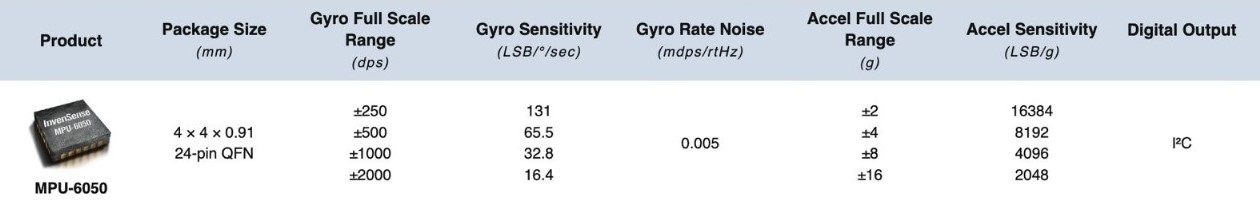
\includegraphics[width=1\linewidth]{Files/Images/Accelerometer.jpg}
    \caption{MPU 6050 Details}
    \label{fig:enter-label}
\end{figure}

\subsection{}